% Options for packages loaded elsewhere
\PassOptionsToPackage{unicode}{hyperref}
\PassOptionsToPackage{hyphens}{url}
%
\documentclass[
  12pt,
  a4paper,
  DIV=11,
  numbers=noendperiod]{scrreprt}

\usepackage{amsmath,amssymb}
\usepackage{setspace}
\usepackage{iftex}
\ifPDFTeX
  \usepackage[T1]{fontenc}
  \usepackage[utf8]{inputenc}
  \usepackage{textcomp} % provide euro and other symbols
\else % if luatex or xetex
  \usepackage{unicode-math}
  \defaultfontfeatures{Scale=MatchLowercase}
  \defaultfontfeatures[\rmfamily]{Ligatures=TeX,Scale=1}
\fi
\usepackage{lmodern}
\ifPDFTeX\else  
    % xetex/luatex font selection
\fi
% Use upquote if available, for straight quotes in verbatim environments
\IfFileExists{upquote.sty}{\usepackage{upquote}}{}
\IfFileExists{microtype.sty}{% use microtype if available
  \usepackage[]{microtype}
  \UseMicrotypeSet[protrusion]{basicmath} % disable protrusion for tt fonts
}{}
\usepackage{xcolor}
\setlength{\emergencystretch}{3em} % prevent overfull lines
\setcounter{secnumdepth}{5}
% Make \paragraph and \subparagraph free-standing
\ifx\paragraph\undefined\else
  \let\oldparagraph\paragraph
  \renewcommand{\paragraph}[1]{\oldparagraph{#1}\mbox{}}
\fi
\ifx\subparagraph\undefined\else
  \let\oldsubparagraph\subparagraph
  \renewcommand{\subparagraph}[1]{\oldsubparagraph{#1}\mbox{}}
\fi

\usepackage{color}
\usepackage{fancyvrb}
\newcommand{\VerbBar}{|}
\newcommand{\VERB}{\Verb[commandchars=\\\{\}]}
\DefineVerbatimEnvironment{Highlighting}{Verbatim}{commandchars=\\\{\}}
% Add ',fontsize=\small' for more characters per line
\usepackage{framed}
\definecolor{shadecolor}{RGB}{241,243,245}
\newenvironment{Shaded}{\begin{snugshade}}{\end{snugshade}}
\newcommand{\AlertTok}[1]{\textcolor[rgb]{0.68,0.00,0.00}{#1}}
\newcommand{\AnnotationTok}[1]{\textcolor[rgb]{0.37,0.37,0.37}{#1}}
\newcommand{\AttributeTok}[1]{\textcolor[rgb]{0.40,0.45,0.13}{#1}}
\newcommand{\BaseNTok}[1]{\textcolor[rgb]{0.68,0.00,0.00}{#1}}
\newcommand{\BuiltInTok}[1]{\textcolor[rgb]{0.00,0.23,0.31}{#1}}
\newcommand{\CharTok}[1]{\textcolor[rgb]{0.13,0.47,0.30}{#1}}
\newcommand{\CommentTok}[1]{\textcolor[rgb]{0.37,0.37,0.37}{#1}}
\newcommand{\CommentVarTok}[1]{\textcolor[rgb]{0.37,0.37,0.37}{\textit{#1}}}
\newcommand{\ConstantTok}[1]{\textcolor[rgb]{0.56,0.35,0.01}{#1}}
\newcommand{\ControlFlowTok}[1]{\textcolor[rgb]{0.00,0.23,0.31}{#1}}
\newcommand{\DataTypeTok}[1]{\textcolor[rgb]{0.68,0.00,0.00}{#1}}
\newcommand{\DecValTok}[1]{\textcolor[rgb]{0.68,0.00,0.00}{#1}}
\newcommand{\DocumentationTok}[1]{\textcolor[rgb]{0.37,0.37,0.37}{\textit{#1}}}
\newcommand{\ErrorTok}[1]{\textcolor[rgb]{0.68,0.00,0.00}{#1}}
\newcommand{\ExtensionTok}[1]{\textcolor[rgb]{0.00,0.23,0.31}{#1}}
\newcommand{\FloatTok}[1]{\textcolor[rgb]{0.68,0.00,0.00}{#1}}
\newcommand{\FunctionTok}[1]{\textcolor[rgb]{0.28,0.35,0.67}{#1}}
\newcommand{\ImportTok}[1]{\textcolor[rgb]{0.00,0.46,0.62}{#1}}
\newcommand{\InformationTok}[1]{\textcolor[rgb]{0.37,0.37,0.37}{#1}}
\newcommand{\KeywordTok}[1]{\textcolor[rgb]{0.00,0.23,0.31}{#1}}
\newcommand{\NormalTok}[1]{\textcolor[rgb]{0.00,0.23,0.31}{#1}}
\newcommand{\OperatorTok}[1]{\textcolor[rgb]{0.37,0.37,0.37}{#1}}
\newcommand{\OtherTok}[1]{\textcolor[rgb]{0.00,0.23,0.31}{#1}}
\newcommand{\PreprocessorTok}[1]{\textcolor[rgb]{0.68,0.00,0.00}{#1}}
\newcommand{\RegionMarkerTok}[1]{\textcolor[rgb]{0.00,0.23,0.31}{#1}}
\newcommand{\SpecialCharTok}[1]{\textcolor[rgb]{0.37,0.37,0.37}{#1}}
\newcommand{\SpecialStringTok}[1]{\textcolor[rgb]{0.13,0.47,0.30}{#1}}
\newcommand{\StringTok}[1]{\textcolor[rgb]{0.13,0.47,0.30}{#1}}
\newcommand{\VariableTok}[1]{\textcolor[rgb]{0.07,0.07,0.07}{#1}}
\newcommand{\VerbatimStringTok}[1]{\textcolor[rgb]{0.13,0.47,0.30}{#1}}
\newcommand{\WarningTok}[1]{\textcolor[rgb]{0.37,0.37,0.37}{\textit{#1}}}

\providecommand{\tightlist}{%
  \setlength{\itemsep}{0pt}\setlength{\parskip}{0pt}}\usepackage{longtable,booktabs,array}
\usepackage{calc} % for calculating minipage widths
% Correct order of tables after \paragraph or \subparagraph
\usepackage{etoolbox}
\makeatletter
\patchcmd\longtable{\par}{\if@noskipsec\mbox{}\fi\par}{}{}
\makeatother
% Allow footnotes in longtable head/foot
\IfFileExists{footnotehyper.sty}{\usepackage{footnotehyper}}{\usepackage{footnote}}
\makesavenoteenv{longtable}
\usepackage{graphicx}
\makeatletter
\def\maxwidth{\ifdim\Gin@nat@width>\linewidth\linewidth\else\Gin@nat@width\fi}
\def\maxheight{\ifdim\Gin@nat@height>\textheight\textheight\else\Gin@nat@height\fi}
\makeatother
% Scale images if necessary, so that they will not overflow the page
% margins by default, and it is still possible to overwrite the defaults
% using explicit options in \includegraphics[width, height, ...]{}
\setkeys{Gin}{width=\maxwidth,height=\maxheight,keepaspectratio}
% Set default figure placement to htbp
\makeatletter
\def\fps@figure{htbp}
\makeatother

\KOMAoption{captions}{tableheading}
\usepackage{indentfirst}
\usepackage{float}
\floatplacement{figure}{H}
\usepackage{libertine}
\makeatletter
\@ifpackageloaded{caption}{}{\usepackage{caption}}
\AtBeginDocument{%
\ifdefined\contentsname
  \renewcommand*\contentsname{Содержание}
\else
  \newcommand\contentsname{Содержание}
\fi
\ifdefined\listfigurename
  \renewcommand*\listfigurename{Список иллюстраций}
\else
  \newcommand\listfigurename{Список иллюстраций}
\fi
\ifdefined\listtablename
  \renewcommand*\listtablename{Список таблиц}
\else
  \newcommand\listtablename{Список таблиц}
\fi
\ifdefined\figurename
  \renewcommand*\figurename{Рисунок}
\else
  \newcommand\figurename{Рисунок}
\fi
\ifdefined\tablename
  \renewcommand*\tablename{Таблица}
\else
  \newcommand\tablename{Таблица}
\fi
}
\@ifpackageloaded{float}{}{\usepackage{float}}
\floatstyle{ruled}
\@ifundefined{c@chapter}{\newfloat{codelisting}{h}{lop}}{\newfloat{codelisting}{h}{lop}[chapter]}
\floatname{codelisting}{Список}
\newcommand*\listoflistings{\listof{codelisting}{Листинги}}
\makeatother
\makeatletter
\makeatother
\makeatletter
\@ifpackageloaded{caption}{}{\usepackage{caption}}
\@ifpackageloaded{subcaption}{}{\usepackage{subcaption}}
\makeatother
\ifLuaTeX
\usepackage[bidi=basic]{babel}
\else
\usepackage[bidi=default]{babel}
\fi
\babelprovide[main,import]{russian}
\babelprovide[import]{english}
% get rid of language-specific shorthands (see #6817):
\let\LanguageShortHands\languageshorthands
\def\languageshorthands#1{}
\ifLuaTeX
  \usepackage{selnolig}  % disable illegal ligatures
\fi
\usepackage[backend=biber,langhook=extras,autolang=other*]{biblatex}
\addbibresource{bib/cite.bib}
\usepackage{csquotes}
\usepackage{bookmark}

\IfFileExists{xurl.sty}{\usepackage{xurl}}{} % add URL line breaks if available
\urlstyle{same} % disable monospaced font for URLs
\hypersetup{
  pdftitle={Лабораторная работа №4},
  pdfauthor={Mohamed Musa},
  pdflang={ru-RU},
  hidelinks,
  pdfcreator={LaTeX via pandoc}}

\title{Лабораторная работа №4}
\usepackage{etoolbox}
\makeatletter
\providecommand{\subtitle}[1]{% add subtitle to \maketitle
  \apptocmd{\@title}{\par {\large #1 \par}}{}{}
}
\makeatother
\subtitle{Настройка современного окружения разработки}
\author{Mohamed Musa}
\date{}

\begin{document}
\maketitle

\renewcommand*\contentsname{Содержание}
{
\setcounter{tocdepth}{1}
\tableofcontents
}
\listoffigures
\listoftables
\setstretch{1.5}
\chapter{Цель
работы}\label{ux446ux435ux43bux44c-ux440ux430ux431ux43eux442ux44b}

Изучить процесс настройки современного окружения разработки с
использованием pnpm, commitizen и conventional commits для управления
проектами.

\chapter{Задание}\label{ux437ux430ux434ux430ux43dux438ux435}

\begin{enumerate}
\def\labelenumi{\arabic{enumi}.}
\tightlist
\item
  Настроить проект с использованием pnpm package manager
\item
  Сконфигурировать commitizen для conventional commits
\item
  Создать package.json с необходимыми зависимостями
\item
  Настроить автоматическое управление changelog
\item
  Создать git репозиторий и выполнить первоначальную настройку
\end{enumerate}

\chapter{Теоретическое
введение}\label{ux442ux435ux43eux440ux435ux442ux438ux447ux435ux441ux43aux43eux435-ux432ux432ux435ux434ux435ux43dux438ux435}

Современная разработка программного обеспечения требует использования
специализированных инструментов для управления зависимостями, контроля
версий и документирования изменений.

\textbf{pnpm} - это эффективный менеджер пакетов для Node.js, который
использует символьные ссылки для экономии дискового пространства и
ускорения установки зависимостей.

\textbf{Commitizen} - инструмент для создания коммитов с соблюдением
conventional commits спецификации, которая обеспечивает единообразие
сообщений коммитов.

\textbf{Conventional Commits} - спецификация для создания понятных
сообщений коммитов с автоматическим семантическим версионированием.

\chapter{Выполнение лабораторной
работы}\label{ux432ux44bux43fux43eux43bux43dux435ux43dux438ux435-ux43bux430ux431ux43eux440ux430ux442ux43eux440ux43dux43eux439-ux440ux430ux431ux43eux442ux44b}

\section{Установка и настройка
pnpm}\label{ux443ux441ux442ux430ux43dux43eux432ux43aux430-ux438-ux43dux430ux441ux442ux440ux43eux439ux43aux430-pnpm}

В начале работы был установлен pnpm package manager. На рисунке
Рисунок~\ref{fig-pnpm} показан процесс настройки проекта с
использованием pnpm.

\begin{figure}

\centering{

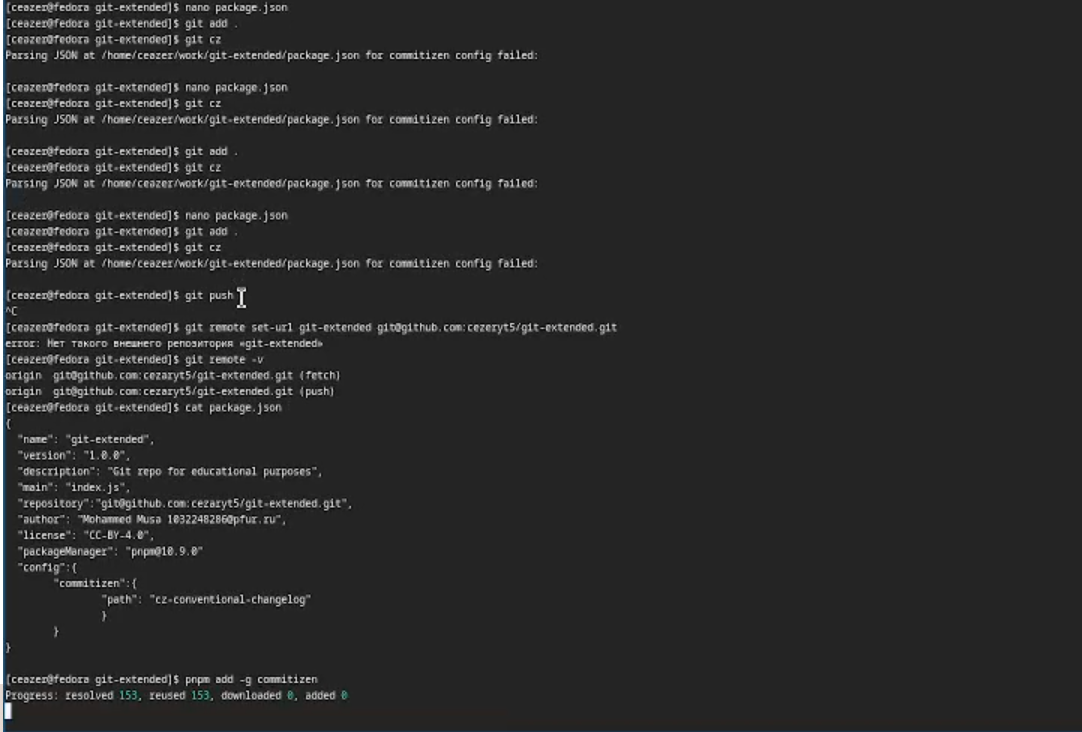
\includegraphics[width=0.8\textwidth,height=\textheight]{image/pnpm.png}

}

\caption{\label{fig-pnpm}Установка и настройка pnpm}

\end{figure}%

\section{Создание
package.json}\label{ux441ux43eux437ux434ux430ux43dux438ux435-package.json}

Был создан файл package.json с необходимой конфигурацией проекта:

\begin{Shaded}
\begin{Highlighting}[]
\FunctionTok{\{}
  \DataTypeTok{"name"}\FunctionTok{:} \StringTok{"git{-}extended"}\FunctionTok{,}
  \DataTypeTok{"version"}\FunctionTok{:} \StringTok{"1.0.0"}\FunctionTok{,}
  \DataTypeTok{"description"}\FunctionTok{:} \StringTok{"Git repo for educational purposes"}\FunctionTok{,}
  \DataTypeTok{"main"}\FunctionTok{:} \StringTok{"index.js"}\FunctionTok{,}
  \DataTypeTok{"scripts"}\FunctionTok{:} \FunctionTok{\{}
    \DataTypeTok{"test"}\FunctionTok{:} \StringTok{"echo }\CharTok{\textbackslash{}"}\StringTok{Error: no test specified}\CharTok{\textbackslash{}"}\StringTok{ \&\& exit 1"}
  \FunctionTok{\},}
  \DataTypeTok{"keywords"}\FunctionTok{:} \OtherTok{[]}\FunctionTok{,}
  \DataTypeTok{"author"}\FunctionTok{:} \StringTok{"Mohamed Musa 1032248286@rudn.ru"}\FunctionTok{,}
  \DataTypeTok{"license"}\FunctionTok{:} \StringTok{"ISC"}\FunctionTok{,}
  \DataTypeTok{"packageManager"}\FunctionTok{:} \StringTok{"pnpm@9.0"}\FunctionTok{,}
  \DataTypeTok{"config"}\FunctionTok{:} \FunctionTok{\{}
    \DataTypeTok{"commitizen"}\FunctionTok{:} \FunctionTok{\{}
      \DataTypeTok{"path"}\FunctionTok{:} \StringTok{"cz{-}conventional{-}changelog"}
    \FunctionTok{\}}
  \FunctionTok{\}}
\FunctionTok{\}}
\end{Highlighting}
\end{Shaded}

Файл package.json показан на рисунке Рисунок~\ref{fig-package-json}.

\begin{figure}

\centering{

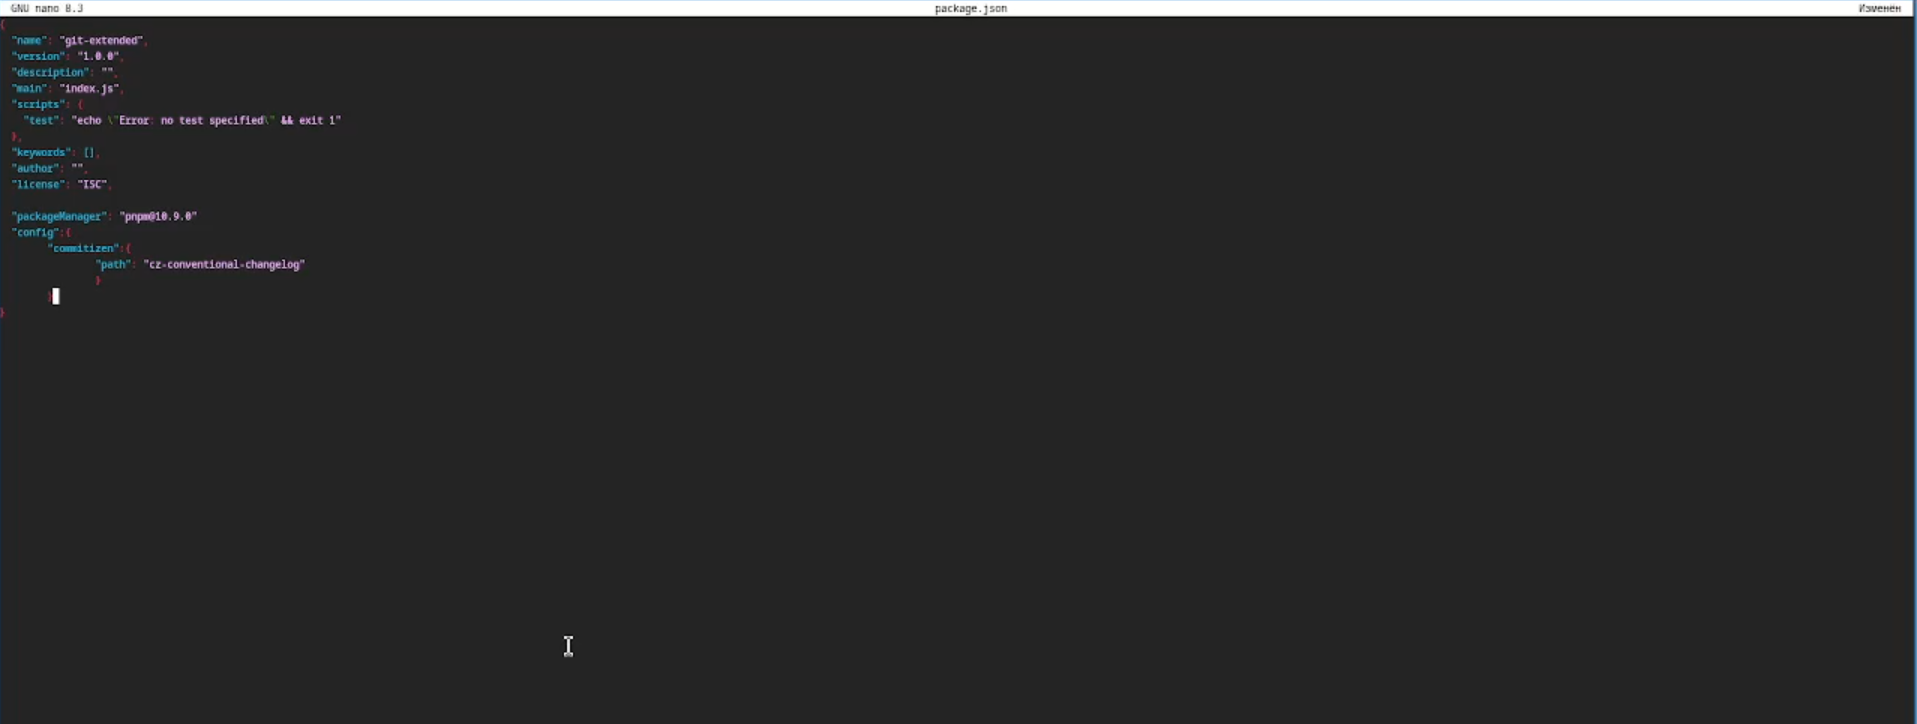
\includegraphics[width=0.8\textwidth,height=\textheight]{image/package.json.png}

}

\caption{\label{fig-package-json}Конфигурация package.json}

\end{figure}%

\section{Установка
commitizen}\label{ux443ux441ux442ux430ux43dux43eux432ux43aux430-commitizen}

Была выполнена установка commitizen с использованием pnpm для создания
conventional commits:

\begin{Shaded}
\begin{Highlighting}[]
\ExtensionTok{pnpm}\NormalTok{ add }\AttributeTok{{-}g}\NormalTok{ commitizen}
\ExtensionTok{pnpm}\NormalTok{ add }\AttributeTok{{-}D}\NormalTok{ cz{-}conventional{-}changelog}
\end{Highlighting}
\end{Shaded}

Процесс установки показан на рисунке Рисунок~\ref{fig-commitzen}.

\begin{figure}

\centering{

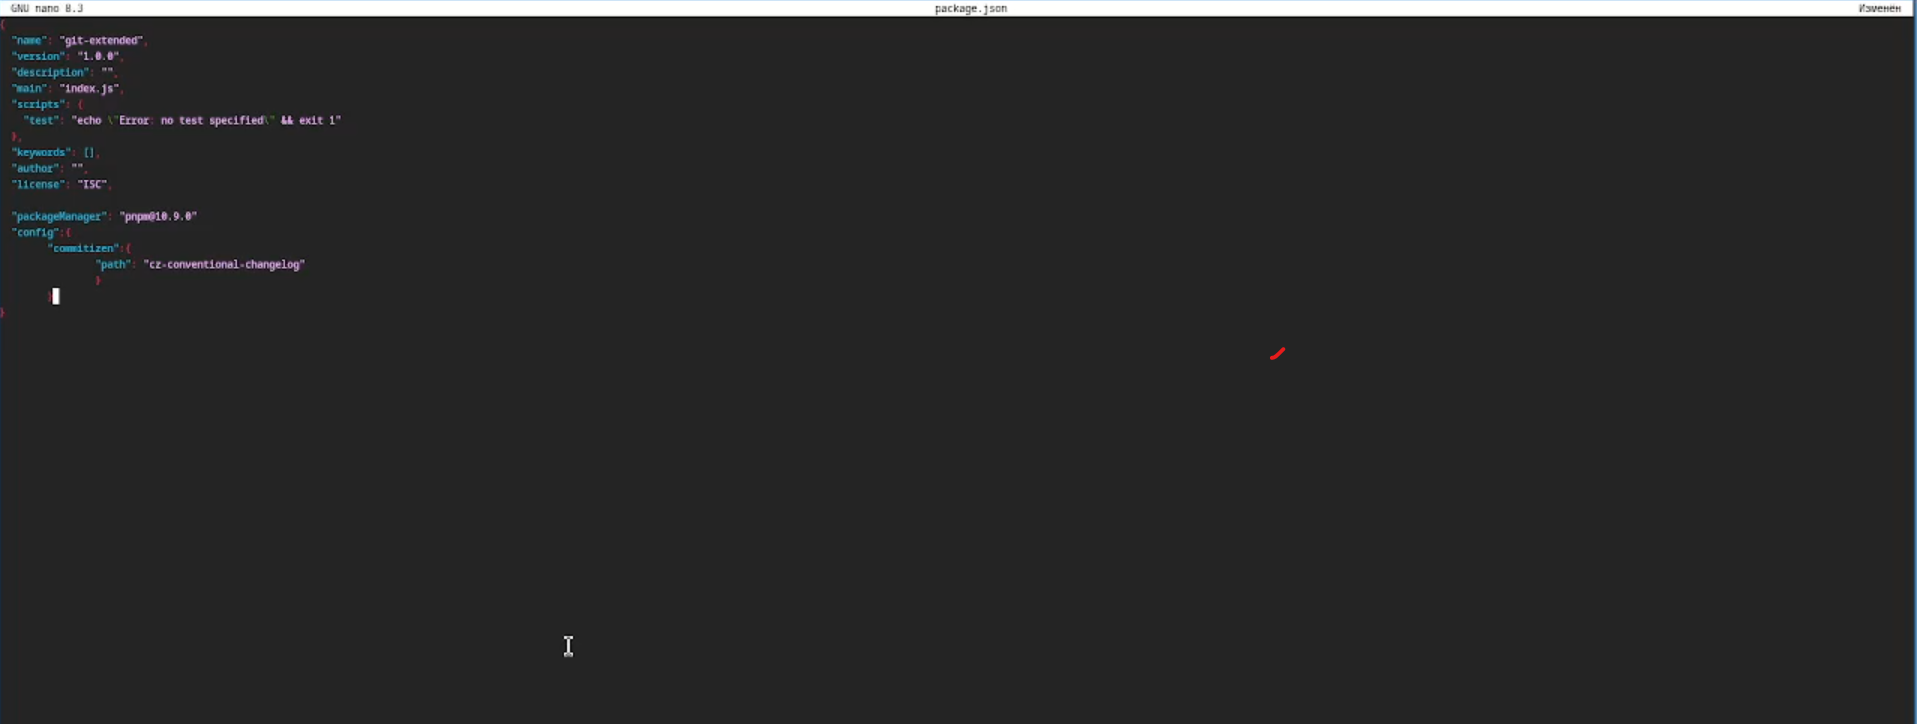
\includegraphics[width=0.8\textwidth,height=\textheight]{image/commitzen.png}

}

\caption{\label{fig-commitzen}Установка commitizen}

\end{figure}%

\section{Создание первого
релиза}\label{ux441ux43eux437ux434ux430ux43dux438ux435-ux43fux435ux440ux432ux43eux433ux43e-ux440ux435ux43bux438ux437ux430}

Был создан первый релиз проекта с использованием стандартных команд git
и npm. На рисунке Рисунок~\ref{fig-release} показан процесс создания
первого релиза.

\begin{figure}

\centering{

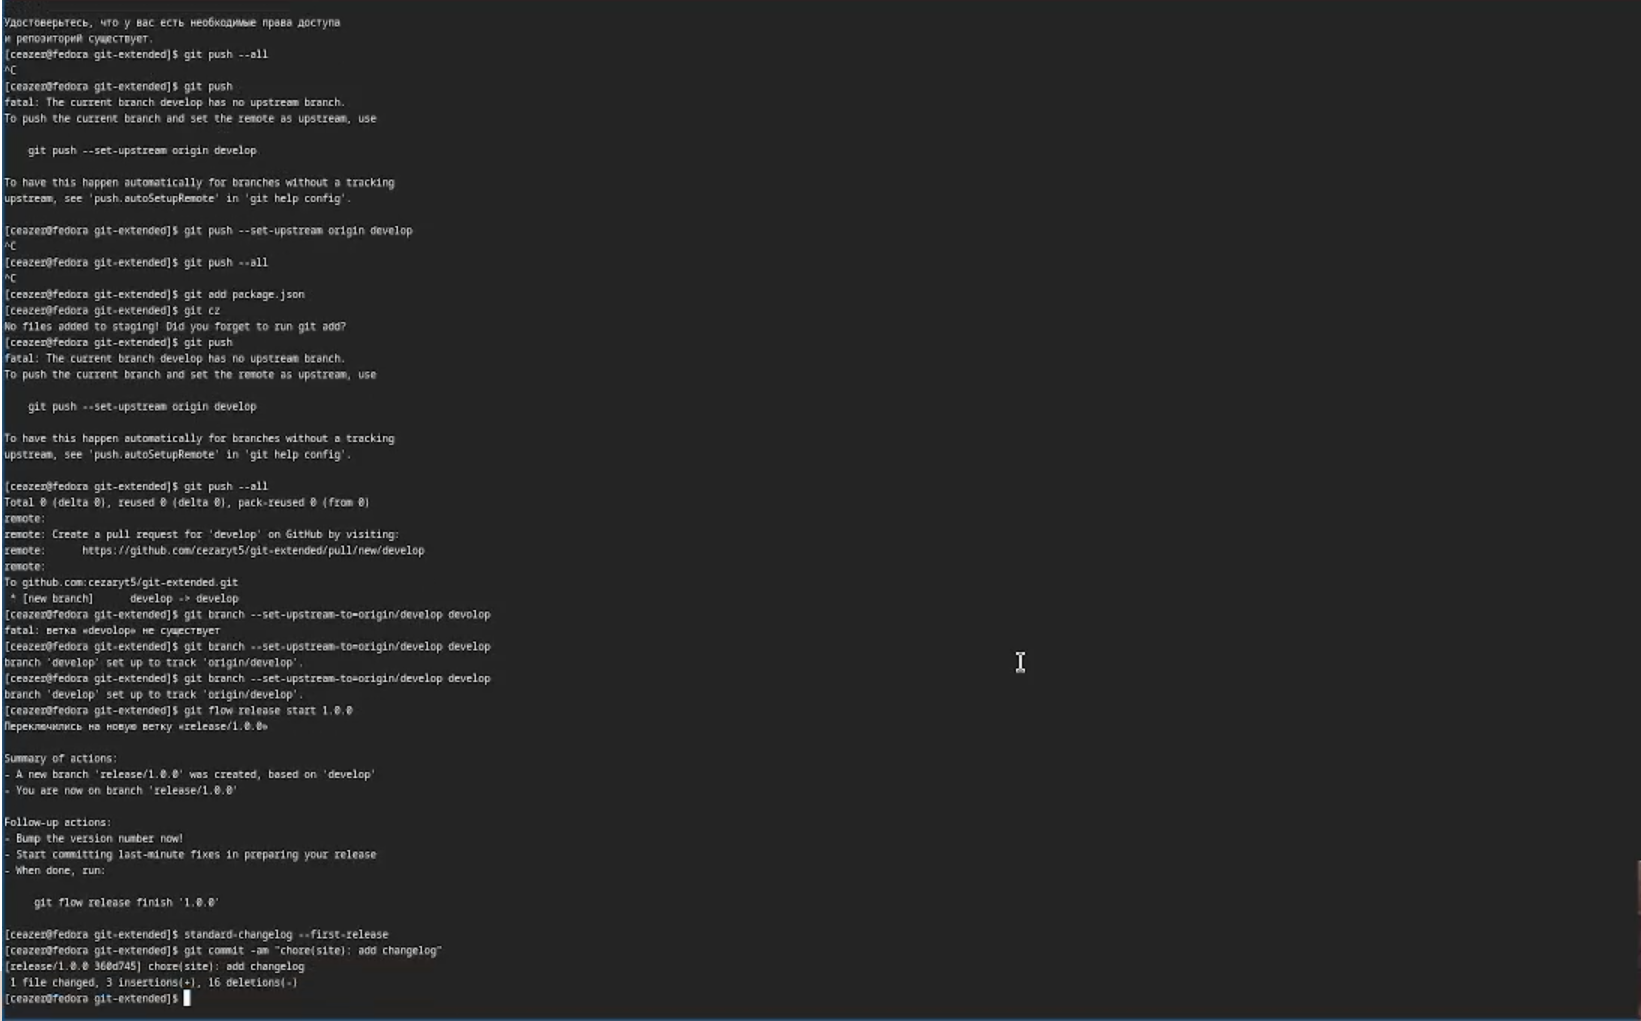
\includegraphics[width=0.8\textwidth,height=\textheight]{image/first release.png}

}

\caption{\label{fig-release}Создание первого релиза}

\end{figure}%

\section{Работа с
changelog}\label{ux440ux430ux431ux43eux442ux430-ux441-changelog}

Были выполнены операции по добавлению записей в changelog и управлению
версиями проекта. Процесс работы с changelog показан на рисунке
Рисунок~\ref{fig-changelog}.

\begin{figure}

\centering{

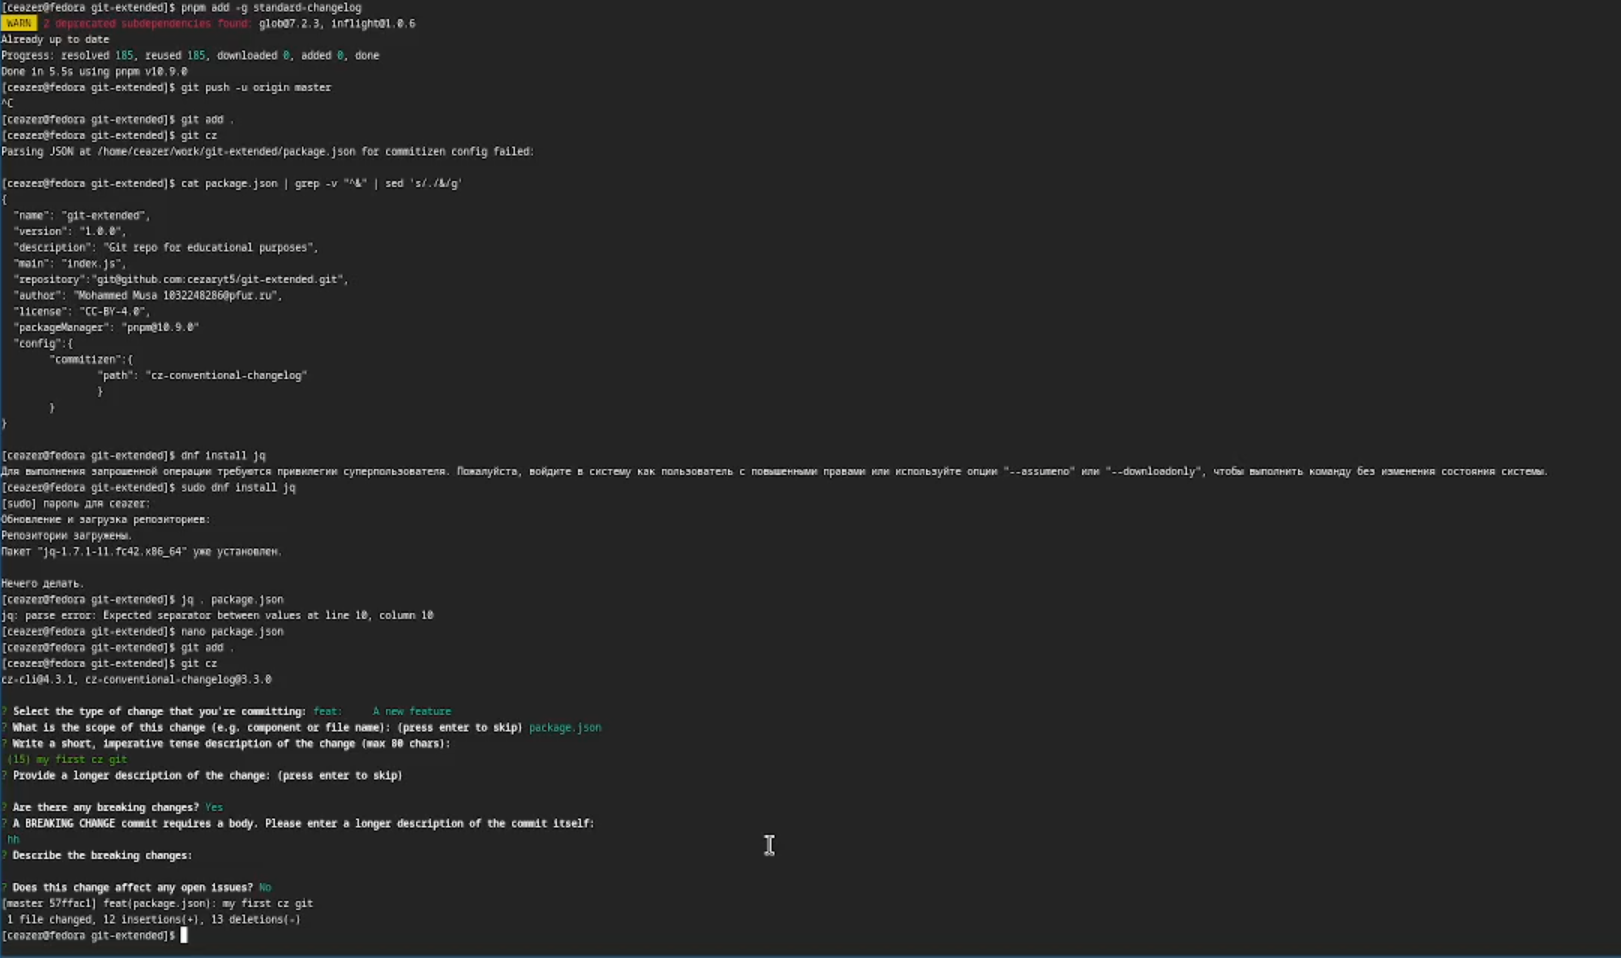
\includegraphics[width=0.8\textwidth,height=\textheight]{image/changelog.png}

}

\caption{\label{fig-changelog}Управление changelog}

\end{figure}%

Дополнительные операции по добавлению в changelog показаны на рисунке
Рисунок~\ref{fig-add-changelog}.

\begin{figure}

\centering{

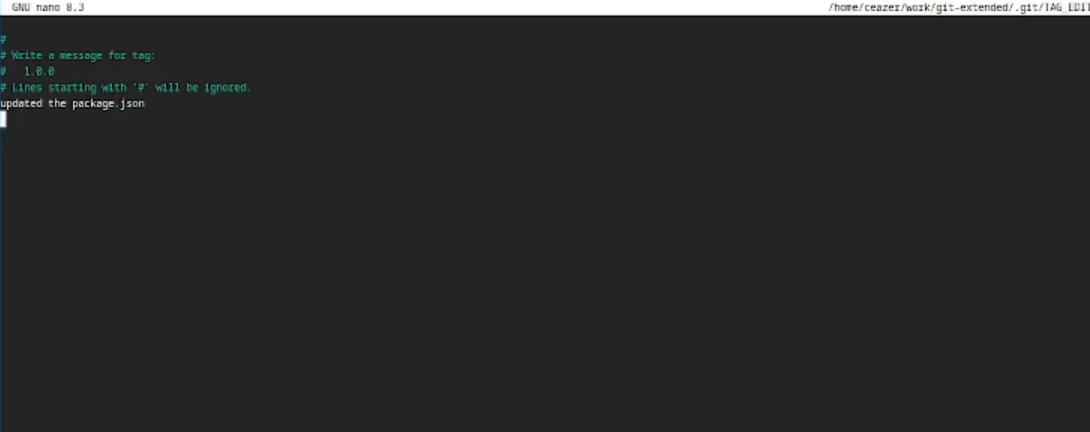
\includegraphics[width=0.8\textwidth,height=\textheight]{image/addChangelog.png}

}

\caption{\label{fig-add-changelog}Добавление в changelog}

\end{figure}%

\section{Выполнение
коммитов}\label{ux432ux44bux43fux43eux43bux43dux435ux43dux438ux435-ux43aux43eux43cux43cux438ux442ux43eux432}

В ходе работы было выполнено несколько коммитов с использованием
настроенного commitizen. Процесс создания коммитов показан на рисунке
Рисунок~\ref{fig-commits}.

\begin{figure}

\centering{

\includegraphics[width=0.8\textwidth,height=\textheight]{image/commits.png}

}

\caption{\label{fig-commits}Создание коммитов с commitizen}

\end{figure}%

\chapter{Выводы}\label{ux432ux44bux432ux43eux434ux44b}

В ходе лабораторной работы были успешно выполнены следующие задачи:

\begin{enumerate}
\def\labelenumi{\arabic{enumi}.}
\tightlist
\item
  ✅ Установлен и настроен pnpm package manager
\item
  ✅ Создан проект git-extended с правильной конфигурацией package.json
\item
  ✅ Настроен commitizen для conventional commits
\item
  ✅ Выполнены операции с git (add, commit, push)
\item
  ✅ Создан и обновлен changelog проекта
\item
  ✅ Выполнен первый релиз проекта
\end{enumerate}

Получены практические навыки работы с современными инструментами
разработки: pnpm для управления зависимостями, commitizen для
стандартизированных коммитов и conventional commits для лучшей
организации процесса разработки.

\chapter*{Список
литературы}\label{ux441ux43fux438ux441ux43eux43a-ux43bux438ux442ux435ux440ux430ux442ux443ux440ux44b}
\addcontentsline{toc}{chapter}{Список литературы}

\printbibliography[heading=none]




\end{document}
